\documentclass[1p]{elsarticle_modified}
%\bibliographystyle{elsarticle-num}

%\usepackage[colorlinks]{hyperref}
%\usepackage{abbrmath_seonhwa} %\Abb, \Ascr, \Acal ,\Abf, \Afrak
\usepackage{amsfonts}
\usepackage{amssymb}
\usepackage{amsmath}
\usepackage{amsthm}
\usepackage{scalefnt}
\usepackage{amsbsy}
\usepackage{kotex}
\usepackage{caption}
\usepackage{subfig}
\usepackage{color}
\usepackage{graphicx}
\usepackage{xcolor} %% white, black, red, green, blue, cyan, magenta, yellow
\usepackage{float}
\usepackage{setspace}
\usepackage{hyperref}

\usepackage{tikz}
\usetikzlibrary{arrows}

\usepackage{multirow}
\usepackage{array} % fixed length table
\usepackage{hhline}

%%%%%%%%%%%%%%%%%%%%%
\makeatletter
\renewcommand*\env@matrix[1][\arraystretch]{%
	\edef\arraystretch{#1}%
	\hskip -\arraycolsep
	\let\@ifnextchar\new@ifnextchar
	\array{*\c@MaxMatrixCols c}}
\makeatother %https://tex.stackexchange.com/questions/14071/how-can-i-increase-the-line-spacing-in-a-matrix
%%%%%%%%%%%%%%%

\usepackage[normalem]{ulem}

\newcommand{\msout}[1]{\ifmmode\text{\sout{\ensuremath{#1}}}\else\sout{#1}\fi}
%SOURCE: \msout is \stkout macro in https://tex.stackexchange.com/questions/20609/strikeout-in-math-mode

\newcommand{\cancel}[1]{
	\ifmmode
	{\color{red}\msout{#1}}
	\else
	{\color{red}\sout{#1}}
	\fi
}

\newcommand{\add}[1]{
	{\color{blue}\uwave{#1}}
}

\newcommand{\replace}[2]{
	\ifmmode
	{\color{red}\msout{#1}}{\color{blue}\uwave{#2}}
	\else
	{\color{red}\sout{#1}}{\color{blue}\uwave{#2}}
	\fi
}

\newcommand{\Sol}{\mathcal{S}} %segment
\newcommand{\D}{D} %diagram
\newcommand{\A}{\mathcal{A}} %arc


%%%%%%%%%%%%%%%%%%%%%%%%%%%%%5 test

\def\sl{\operatorname{\textup{SL}}(2,\Cbb)}
\def\psl{\operatorname{\textup{PSL}}(2,\Cbb)}
\def\quan{\mkern 1mu \triangleright \mkern 1mu}

\theoremstyle{definition}
\newtheorem{thm}{Theorem}[section]
\newtheorem{prop}[thm]{Proposition}
\newtheorem{lem}[thm]{Lemma}
\newtheorem{ques}[thm]{Question}
\newtheorem{cor}[thm]{Corollary}
\newtheorem{defn}[thm]{Definition}
\newtheorem{exam}[thm]{Example}
\newtheorem{rmk}[thm]{Remark}
\newtheorem{alg}[thm]{Algorithm}

\newcommand{\I}{\sqrt{-1}}
\begin{document}

%\begin{frontmatter}
%
%\title{Boundary parabolic representations of knots up to 8 crossings}
%
%%% Group authors per affiliation:
%\author{Yunhi Cho} 
%\address{Department of Mathematics, University of Seoul, Seoul, Korea}
%\ead{yhcho@uos.ac.kr}
%
%
%\author{Seonhwa Kim} %\fnref{s_kim}}
%\address{Center for Geometry and Physics, Institute for Basic Science, Pohang, 37673, Korea}
%\ead{ryeona17@ibs.re.kr}
%
%\author{Hyuk Kim}
%\address{Department of Mathematical Sciences, Seoul National University, Seoul 08826, Korea}
%\ead{hyukkim@snu.ac.kr}
%
%\author{Seokbeom Yoon}
%\address{Department of Mathematical Sciences, Seoul National University, Seoul, 08826,  Korea}
%\ead{sbyoon15@snu.ac.kr}
%
%\begin{abstract}
%We find all boundary parabolic representation of knots up to 8 crossings.
%
%\end{abstract}
%\begin{keyword}
%    \MSC[2010] 57M25 
%\end{keyword}
%
%\end{frontmatter}

%\linenumbers
%\tableofcontents
%
\newcommand\colored[1]{\textcolor{white}{\rule[-0.35ex]{0.8em}{1.4ex}}\kern-0.8em\color{red} #1}%
%\newcommand\colored[1]{\textcolor{white}{ #1}\kern-2.17ex	\textcolor{white}{ #1}\kern-1.81ex	\textcolor{white}{ #1}\kern-2.15ex\color{red}#1	}

{\Large $\underline{11a_{80}~(K11a_{80})}$}

\setlength{\tabcolsep}{10pt}
\renewcommand{\arraystretch}{1.6}
\vspace{1cm}\begin{tabular}{m{100pt}>{\centering\arraybackslash}m{274pt}}
\multirow{5}{120pt}{
	\centering
	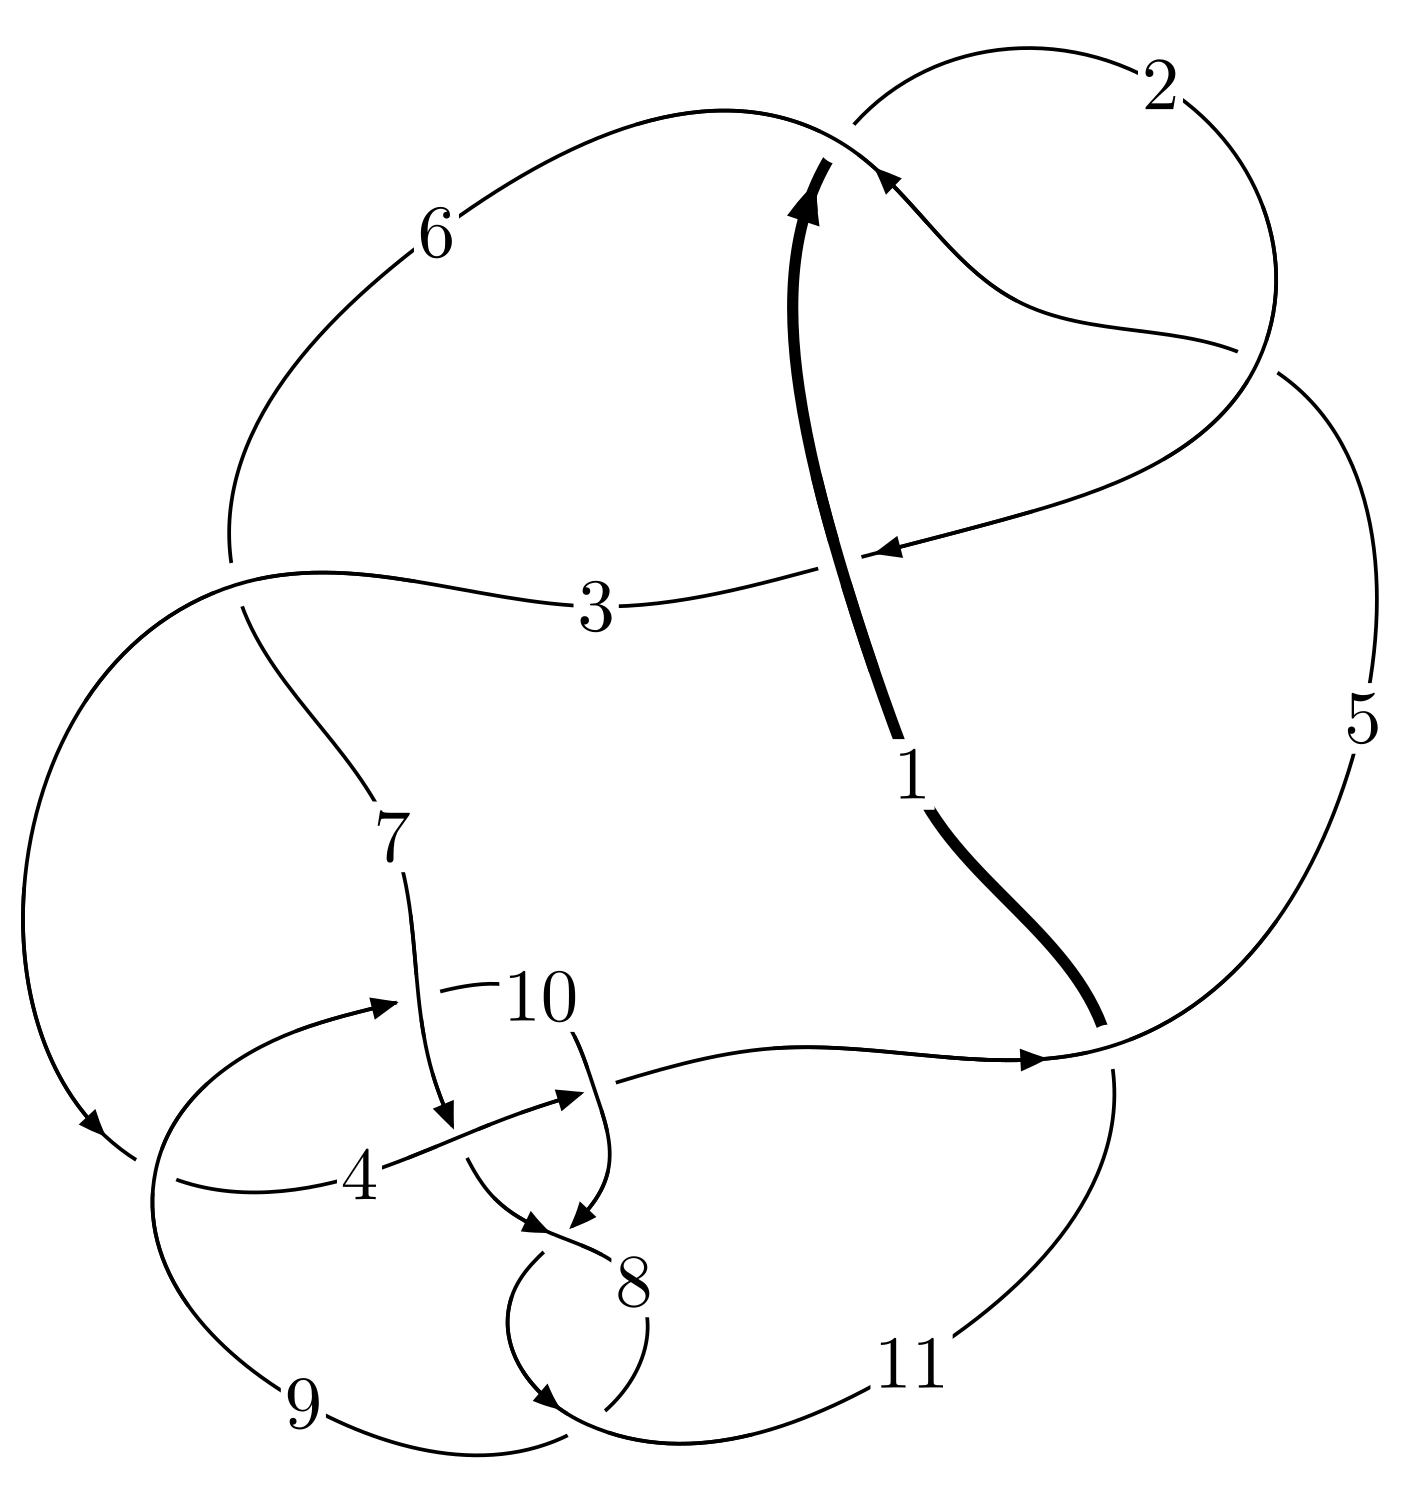
\includegraphics[width=112pt]{../../../GIT/diagram.site/Diagrams/png/329_11a_80.png}\\
\ \ \ A knot diagram\footnotemark}&
\allowdisplaybreaks
\textbf{Linearized knot diagam} \\
\cline{2-2}
 &
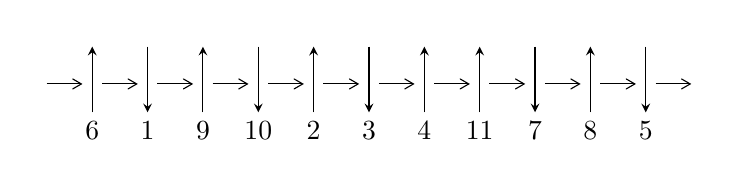
\begin{tikzpicture}[x=20pt, y=17pt]
	% nodes
	\node (C0) at (0, 0) {};
	\node (C1) at (1, 0) {};
	\node (C1U) at (1, +1) {};
	\node (C1D) at (1, -1) {6};

	\node (C2) at (2, 0) {};
	\node (C2U) at (2, +1) {};
	\node (C2D) at (2, -1) {1};

	\node (C3) at (3, 0) {};
	\node (C3U) at (3, +1) {};
	\node (C3D) at (3, -1) {9};

	\node (C4) at (4, 0) {};
	\node (C4U) at (4, +1) {};
	\node (C4D) at (4, -1) {10};

	\node (C5) at (5, 0) {};
	\node (C5U) at (5, +1) {};
	\node (C5D) at (5, -1) {2};

	\node (C6) at (6, 0) {};
	\node (C6U) at (6, +1) {};
	\node (C6D) at (6, -1) {3};

	\node (C7) at (7, 0) {};
	\node (C7U) at (7, +1) {};
	\node (C7D) at (7, -1) {4};

	\node (C8) at (8, 0) {};
	\node (C8U) at (8, +1) {};
	\node (C8D) at (8, -1) {11};

	\node (C9) at (9, 0) {};
	\node (C9U) at (9, +1) {};
	\node (C9D) at (9, -1) {7};

	\node (C10) at (10, 0) {};
	\node (C10U) at (10, +1) {};
	\node (C10D) at (10, -1) {8};

	\node (C11) at (11, 0) {};
	\node (C11U) at (11, +1) {};
	\node (C11D) at (11, -1) {5};
	\node (C12) at (12, 0) {};

	% arrows
	\draw[->,>={angle 60}]
	(C0) edge (C1) (C1) edge (C2) (C2) edge (C3) (C3) edge (C4) (C4) edge (C5) (C5) edge (C6) (C6) edge (C7) (C7) edge (C8) (C8) edge (C9) (C9) edge (C10) (C10) edge (C11) (C11) edge (C12) ;	\draw[->,>=stealth]
	(C1D) edge (C1U) (C2U) edge (C2D) (C3D) edge (C3U) (C4U) edge (C4D) (C5D) edge (C5U) (C6U) edge (C6D) (C7D) edge (C7U) (C8D) edge (C8U) (C9U) edge (C9D) (C10D) edge (C10U) (C11U) edge (C11D) ;
	\end{tikzpicture} \\
\hhline{~~} \\& 
\textbf{Solving Sequence} \\ \cline{2-2} 
 &
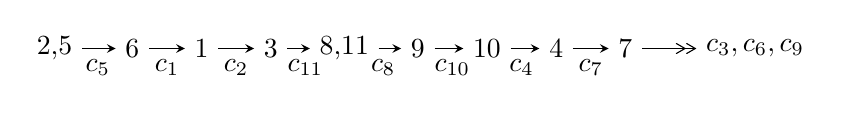
\begin{tikzpicture}[x=25pt, y=7pt]
	% node
	\node (A0) at (-1/8, 0) {2,5};
	\node (A1) at (1, 0) {6};
	\node (A2) at (2, 0) {1};
	\node (A3) at (3, 0) {3};
	\node (A4) at (65/16, 0) {8,11};
	\node (A5) at (41/8, 0) {9};
	\node (A6) at (49/8, 0) {10};
	\node (A7) at (57/8, 0) {4};
	\node (A8) at (65/8, 0) {7};
	\node (C1) at (1/2, -1) {$c_{5}$};
	\node (C2) at (3/2, -1) {$c_{1}$};
	\node (C3) at (5/2, -1) {$c_{2}$};
	\node (C4) at (7/2, -1) {$c_{11}$};
	\node (C5) at (37/8, -1) {$c_{8}$};
	\node (C6) at (45/8, -1) {$c_{10}$};
	\node (C7) at (53/8, -1) {$c_{4}$};
	\node (C8) at (61/8, -1) {$c_{7}$};
	\node (A9) at (10, 0) {$c_{3},c_{6},c_{9}$};

	% edge
	\draw[->,>=stealth]	
	(A0) edge (A1) (A1) edge (A2) (A2) edge (A3) (A3) edge (A4) (A4) edge (A5) (A5) edge (A6) (A6) edge (A7) (A7) edge (A8) ;
	\draw[->>,>={angle 60}]	
	(A8) edge (A9);
\end{tikzpicture} \\ 

\end{tabular} \\

\footnotetext{
The image of knot diagram is generated by the software ``\textbf{Draw programme}" developed by Andrew Bartholomew(\url{http://www.layer8.co.uk/maths/draw/index.htm\#Running-draw}), where we modified some parts for our purpose(\url{https://github.com/CATsTAILs/LinksPainter}).
}\phantom \\ \newline 
\centering \textbf{Ideals for irreducible components\footnotemark of $X_{\text{par}}$} 
 
\begin{align*}
I^u_{1}&=\langle 
-1.10807\times10^{23} u^{69}+2.13624\times10^{23} u^{68}+\cdots+3.25909\times10^{22} b+1.02987\times10^{23},\\
\phantom{I^u_{1}}&\phantom{= \langle  }7.69171\times10^{22} u^{69}-4.41119\times10^{22} u^{68}+\cdots+3.25909\times10^{22} a-4.48719\times10^{22},\;u^{70}-2 u^{69}+\cdots-5 u+1\rangle \\
I^u_{2}&=\langle 
b+2 u-1,\;a-2,\;u^2- u+1\rangle \\
\\
\end{align*}
\raggedright * 2 irreducible components of $\dim_{\mathbb{C}}=0$, with total 72 representations.\\
\footnotetext{All coefficients of polynomials are rational numbers. But the coefficients are sometimes approximated in decimal forms when there is not enough margin.}
\newpage
\renewcommand{\arraystretch}{1}
\centering \section*{I. $I^u_{1}= \langle -1.11\times10^{23} u^{69}+2.14\times10^{23} u^{68}+\cdots+3.26\times10^{22} b+1.03\times10^{23},\;7.69\times10^{22} u^{69}-4.41\times10^{22} u^{68}+\cdots+3.26\times10^{22} a-4.49\times10^{22},\;u^{70}-2 u^{69}+\cdots-5 u+1 \rangle$}
\flushleft \textbf{(i) Arc colorings}\\
\begin{tabular}{m{7pt} m{180pt} m{7pt} m{180pt} }
\flushright $a_{2}=$&$\begin{pmatrix}0\\u\end{pmatrix}$ \\
\flushright $a_{5}=$&$\begin{pmatrix}1\\0\end{pmatrix}$ \\
\flushright $a_{6}=$&$\begin{pmatrix}1\\- u^2\end{pmatrix}$ \\
\flushright $a_{1}=$&$\begin{pmatrix}- u\\u^3+u\end{pmatrix}$ \\
\flushright $a_{3}=$&$\begin{pmatrix}- u^3\\u^5+u^3+u\end{pmatrix}$ \\
\flushright $a_{8}=$&$\begin{pmatrix}-2.36008 u^{69}+1.35350 u^{68}+\cdots+2.96444 u+1.37682\\3.39992 u^{69}-6.55471 u^{68}+\cdots+15.8232 u-3.16000\end{pmatrix}$ \\
\flushright $a_{11}=$&$\begin{pmatrix}u^3\\u^3+u\end{pmatrix}$ \\
\flushright $a_{9}=$&$\begin{pmatrix}-2.36035 u^{69}+1.58814 u^{68}+\cdots+2.07836 u+1.59404\\3.19965 u^{69}-6.13729 u^{68}+\cdots+14.0060 u-2.96000\end{pmatrix}$ \\
\flushright $a_{10}=$&$\begin{pmatrix}2.55997 u^{69}-1.82063 u^{68}+\cdots-3.25615 u-1.70993\\-3.20003 u^{69}+6.36373 u^{68}+\cdots-14.8901 u+3.16000\end{pmatrix}$ \\
\flushright $a_{4}=$&$\begin{pmatrix}6.40571 u^{69}-13.1764 u^{68}+\cdots+34.5221 u-3.44819\\1.36498 u^{69}+3.63005 u^{68}+\cdots-22.5376 u+5.79503\end{pmatrix}$ \\
\flushright $a_{7}=$&$\begin{pmatrix}- u^6- u^4+1\\u^8+2 u^6+2 u^4\end{pmatrix}$\\ \flushright $a_{7}=$&$\begin{pmatrix}- u^6- u^4+1\\u^8+2 u^6+2 u^4\end{pmatrix}$\\&\end{tabular}
\flushleft \textbf{(ii) Obstruction class $= -1$}\\~\\
\flushleft \textbf{(iii) Cusp Shapes $= \frac{80166540663254872590873}{10863644501129272985843} u^{69}-\frac{390207808448510879557707}{10863644501129272985843} u^{68}+\cdots+\frac{1547885087409440226722281}{10863644501129272985843} u-\frac{321339458068418410398408}{10863644501129272985843}$}\\~\\
\newpage\renewcommand{\arraystretch}{1}
\flushleft \textbf{(iv) u-Polynomials at the component}\newline \\
\begin{tabular}{m{50pt}|m{274pt}}
Crossings & \hspace{64pt}u-Polynomials at each crossing \\
\hline $$\begin{aligned}c_{1},c_{5}\end{aligned}$$&$\begin{aligned}
&u^{70}-2 u^{69}+\cdots-5 u+1
\end{aligned}$\\
\hline $$\begin{aligned}c_{2}\end{aligned}$$&$\begin{aligned}
&u^{70}+38 u^{69}+\cdots- u+1
\end{aligned}$\\
\hline $$\begin{aligned}c_{3}\end{aligned}$$&$\begin{aligned}
&u^{70}+2 u^{69}+\cdots+23 u+107
\end{aligned}$\\
\hline $$\begin{aligned}c_{4}\end{aligned}$$&$\begin{aligned}
&u^{70}+31 u^{68}+\cdots-13 u+1
\end{aligned}$\\
\hline $$\begin{aligned}c_{6},c_{11}\end{aligned}$$&$\begin{aligned}
&u^{70}+2 u^{69}+\cdots-169 u+17
\end{aligned}$\\
\hline $$\begin{aligned}c_{7}\end{aligned}$$&$\begin{aligned}
&u^{70}-2 u^{69}+\cdots- u+1
\end{aligned}$\\
\hline $$\begin{aligned}c_{8},c_{10}\end{aligned}$$&$\begin{aligned}
&u^{70}+3 u^{69}+\cdots-4 u+1
\end{aligned}$\\
\hline $$\begin{aligned}c_{9}\end{aligned}$$&$\begin{aligned}
&u^{70}-11 u^{69}+\cdots+4 u+4
\end{aligned}$\\
\hline
\end{tabular}\\~\\
\newpage\renewcommand{\arraystretch}{1}
\flushleft \textbf{(v) Riley Polynomials at the component}\newline \\
\begin{tabular}{m{50pt}|m{274pt}}
Crossings & \hspace{64pt}Riley Polynomials at each crossing \\
\hline $$\begin{aligned}c_{1},c_{5}\end{aligned}$$&$\begin{aligned}
&y^{70}+38 y^{69}+\cdots- y+1
\end{aligned}$\\
\hline $$\begin{aligned}c_{2}\end{aligned}$$&$\begin{aligned}
&y^{70}-10 y^{69}+\cdots-93 y+1
\end{aligned}$\\
\hline $$\begin{aligned}c_{3}\end{aligned}$$&$\begin{aligned}
&y^{70}+70 y^{69}+\cdots+344439 y+11449
\end{aligned}$\\
\hline $$\begin{aligned}c_{4}\end{aligned}$$&$\begin{aligned}
&y^{70}+62 y^{69}+\cdots+127 y+1
\end{aligned}$\\
\hline $$\begin{aligned}c_{6},c_{11}\end{aligned}$$&$\begin{aligned}
&y^{70}-58 y^{69}+\cdots-16865 y+289
\end{aligned}$\\
\hline $$\begin{aligned}c_{7}\end{aligned}$$&$\begin{aligned}
&y^{70}-10 y^{69}+\cdots- y+1
\end{aligned}$\\
\hline $$\begin{aligned}c_{8},c_{10}\end{aligned}$$&$\begin{aligned}
&y^{70}-41 y^{69}+\cdots+16 y+1
\end{aligned}$\\
\hline $$\begin{aligned}c_{9}\end{aligned}$$&$\begin{aligned}
&y^{70}-15 y^{69}+\cdots-200 y+16
\end{aligned}$\\
\hline
\end{tabular}\\~\\
\newpage\flushleft \textbf{(vi) Complex Volumes and Cusp Shapes}
$$\begin{array}{c|c|c}  
\text{Solutions to }I^u_{1}& \I (\text{vol} + \sqrt{-1}CS) & \text{Cusp shape}\\
 \hline 
\begin{aligned}
u &= \phantom{-}0.629527 + 0.806981 I \\
a &= \phantom{-}1.41570 - 0.09923 I \\
b &= \phantom{-}0.33030 - 1.77174 I\end{aligned}
 & \phantom{-}1.04825 + 2.45107 I & \phantom{-0.000000 } 0 \\ \hline\begin{aligned}
u &= \phantom{-}0.629527 - 0.806981 I \\
a &= \phantom{-}1.41570 + 0.09923 I \\
b &= \phantom{-}0.33030 + 1.77174 I\end{aligned}
 & \phantom{-}1.04825 - 2.45107 I & \phantom{-0.000000 } 0 \\ \hline\begin{aligned}
u &= -0.067651 + 1.027570 I \\
a &= \phantom{-}0.485648 + 1.262690 I \\
b &= \phantom{-}0.577177 + 0.334792 I\end{aligned}
 & -3.59009 + 0.96831 I & \phantom{-0.000000 } 0 \\ \hline\begin{aligned}
u &= -0.067651 - 1.027570 I \\
a &= \phantom{-}0.485648 - 1.262690 I \\
b &= \phantom{-}0.577177 - 0.334792 I\end{aligned}
 & -3.59009 - 0.96831 I & \phantom{-0.000000 } 0 \\ \hline\begin{aligned}
u &= \phantom{-}0.384830 + 0.888904 I \\
a &= \phantom{-}0.644025 + 0.369584 I \\
b &= \phantom{-}0.586602 - 0.314795 I\end{aligned}
 & -0.32453 + 1.95228 I & \phantom{-0.000000 } 0. - 3.30692 I \\ \hline\begin{aligned}
u &= \phantom{-}0.384830 - 0.888904 I \\
a &= \phantom{-}0.644025 - 0.369584 I \\
b &= \phantom{-}0.586602 + 0.314795 I\end{aligned}
 & -0.32453 - 1.95228 I & \phantom{-0.000000 -}0. + 3.30692 I \\ \hline\begin{aligned}
u &= -0.479076 + 0.914334 I \\
a &= -0.835502 - 0.636450 I \\
b &= -0.0502703 - 0.0626528 I\end{aligned}
 & -0.79732 - 5.73779 I & \phantom{-0.000000 } 0 \\ \hline\begin{aligned}
u &= -0.479076 - 0.914334 I \\
a &= -0.835502 + 0.636450 I \\
b &= -0.0502703 + 0.0626528 I\end{aligned}
 & -0.79732 + 5.73779 I & \phantom{-0.000000 } 0 \\ \hline\begin{aligned}
u &= -0.463852 + 0.816066 I \\
a &= \phantom{-}1.03712 - 1.14502 I \\
b &= -0.065861 + 1.165360 I\end{aligned}
 & \phantom{-}3.32585 - 3.64623 I & \phantom{-}8.36983 + 8.12955 I \\ \hline\begin{aligned}
u &= -0.463852 - 0.816066 I \\
a &= \phantom{-}1.03712 + 1.14502 I \\
b &= -0.065861 - 1.165360 I\end{aligned}
 & \phantom{-}3.32585 + 3.64623 I & \phantom{-}8.36983 - 8.12955 I\\
 \hline 
 \end{array}$$\newpage$$\begin{array}{c|c|c}  
\text{Solutions to }I^u_{1}& \I (\text{vol} + \sqrt{-1}CS) & \text{Cusp shape}\\
 \hline 
\begin{aligned}
u &= -0.584393 + 0.923619 I \\
a &= -2.09703 + 0.21211 I \\
b &= -0.57442 - 1.93822 I\end{aligned}
 & \phantom{-}3.25750 - 10.82580 I & \phantom{-0.000000 } 0 \\ \hline\begin{aligned}
u &= -0.584393 - 0.923619 I \\
a &= -2.09703 - 0.21211 I \\
b &= -0.57442 + 1.93822 I\end{aligned}
 & \phantom{-}3.25750 + 10.82580 I & \phantom{-0.000000 } 0 \\ \hline\begin{aligned}
u &= \phantom{-}0.377490 + 0.808869 I \\
a &= -4.46362 - 0.46805 I \\
b &= \phantom{-}0.09813 + 3.87415 I\end{aligned}
 & \phantom{-}1.50422 + 1.66288 I & -31.1505 + 27.2219 I \\ \hline\begin{aligned}
u &= \phantom{-}0.377490 - 0.808869 I \\
a &= -4.46362 + 0.46805 I \\
b &= \phantom{-}0.09813 - 3.87415 I\end{aligned}
 & \phantom{-}1.50422 - 1.66288 I & -31.1505 - 27.2219 I \\ \hline\begin{aligned}
u &= -0.653862 + 0.578775 I \\
a &= -0.775452 + 0.290765 I \\
b &= \phantom{-}0.31099 - 1.84334 I\end{aligned}
 & \phantom{-}4.24693 + 6.03843 I & \phantom{-}5.38503 - 4.49312 I \\ \hline\begin{aligned}
u &= -0.653862 - 0.578775 I \\
a &= -0.775452 - 0.290765 I \\
b &= \phantom{-}0.31099 + 1.84334 I\end{aligned}
 & \phantom{-}4.24693 - 6.03843 I & \phantom{-}5.38503 + 4.49312 I \\ \hline\begin{aligned}
u &= \phantom{-}0.851538 + 0.139959 I \\
a &= -1.044180 - 0.205566 I \\
b &= -1.12487 - 1.81917 I\end{aligned}
 & -0.99836 - 11.50700 I & \phantom{-}1.84093 + 6.73084 I \\ \hline\begin{aligned}
u &= \phantom{-}0.851538 - 0.139959 I \\
a &= -1.044180 + 0.205566 I \\
b &= -1.12487 + 1.81917 I\end{aligned}
 & -0.99836 + 11.50700 I & \phantom{-}1.84093 - 6.73084 I \\ \hline\begin{aligned}
u &= \phantom{-}0.060029 + 1.146880 I \\
a &= -0.18745 + 2.16143 I \\
b &= -0.299074 + 1.201650 I\end{aligned}
 & -1.44288 + 5.44607 I & \phantom{-0.000000 } 0 \\ \hline\begin{aligned}
u &= \phantom{-}0.060029 - 1.146880 I \\
a &= -0.18745 - 2.16143 I \\
b &= -0.299074 - 1.201650 I\end{aligned}
 & -1.44288 - 5.44607 I & \phantom{-0.000000 } 0\\
 \hline 
 \end{array}$$\newpage$$\begin{array}{c|c|c}  
\text{Solutions to }I^u_{1}& \I (\text{vol} + \sqrt{-1}CS) & \text{Cusp shape}\\
 \hline 
\begin{aligned}
u &= -0.830885 + 0.169788 I \\
a &= \phantom{-}0.885873 - 0.209106 I \\
b &= \phantom{-}1.24593 - 1.41968 I\end{aligned}
 & -2.35547 + 3.73849 I & -0.65968 - 5.52505 I \\ \hline\begin{aligned}
u &= -0.830885 - 0.169788 I \\
a &= \phantom{-}0.885873 + 0.209106 I \\
b &= \phantom{-}1.24593 + 1.41968 I\end{aligned}
 & -2.35547 - 3.73849 I & -0.65968 + 5.52505 I \\ \hline\begin{aligned}
u &= -0.844269 + 0.045265 I \\
a &= \phantom{-}0.529036 - 0.217259 I \\
b &= \phantom{-}0.438531 + 0.049854 I\end{aligned}
 & -3.62841 + 0.20387 I & -2.37460 + 1.94241 I \\ \hline\begin{aligned}
u &= -0.844269 - 0.045265 I \\
a &= \phantom{-}0.529036 + 0.217259 I \\
b &= \phantom{-}0.438531 - 0.049854 I\end{aligned}
 & -3.62841 - 0.20387 I & -2.37460 - 1.94241 I \\ \hline\begin{aligned}
u &= \phantom{-}0.696611 + 0.477869 I \\
a &= -0.242169 + 0.044656 I \\
b &= -0.23295 - 1.56391 I\end{aligned}
 & \phantom{-}3.77878 + 3.85148 I & \phantom{-}5.41405 - 7.02923 I \\ \hline\begin{aligned}
u &= \phantom{-}0.696611 - 0.477869 I \\
a &= -0.242169 - 0.044656 I \\
b &= -0.23295 + 1.56391 I\end{aligned}
 & \phantom{-}3.77878 - 3.85148 I & \phantom{-}5.41405 + 7.02923 I \\ \hline\begin{aligned}
u &= -0.441288 + 0.716327 I \\
a &= \phantom{-}1.55504 - 1.61375 I \\
b &= \phantom{-}0.220804 + 0.919376 I\end{aligned}
 & \phantom{-}3.62277 - 0.21985 I & \phantom{-}9.90987 + 0.81181 I \\ \hline\begin{aligned}
u &= -0.441288 - 0.716327 I \\
a &= \phantom{-}1.55504 + 1.61375 I \\
b &= \phantom{-}0.220804 - 0.919376 I\end{aligned}
 & \phantom{-}3.62277 + 0.21985 I & \phantom{-}9.90987 - 0.81181 I \\ \hline\begin{aligned}
u &= \phantom{-}0.589180 + 1.012730 I \\
a &= \phantom{-}2.20968 - 0.22515 I \\
b &= \phantom{-}0.60519 - 1.40546 I\end{aligned}
 & \phantom{-}2.24373 + 1.06051 I & \phantom{-0.000000 } 0 \\ \hline\begin{aligned}
u &= \phantom{-}0.589180 - 1.012730 I \\
a &= \phantom{-}2.20968 + 0.22515 I \\
b &= \phantom{-}0.60519 + 1.40546 I\end{aligned}
 & \phantom{-}2.24373 - 1.06051 I & \phantom{-0.000000 } 0\\
 \hline 
 \end{array}$$\newpage$$\begin{array}{c|c|c}  
\text{Solutions to }I^u_{1}& \I (\text{vol} + \sqrt{-1}CS) & \text{Cusp shape}\\
 \hline 
\begin{aligned}
u &= \phantom{-}0.816520 + 0.092061 I \\
a &= -0.246027 - 0.625616 I \\
b &= \phantom{-}0.227076 + 0.411053 I\end{aligned}
 & -4.47780 - 5.27299 I & -1.13386 + 5.09920 I \\ \hline\begin{aligned}
u &= \phantom{-}0.816520 - 0.092061 I \\
a &= -0.246027 + 0.625616 I \\
b &= \phantom{-}0.227076 - 0.411053 I\end{aligned}
 & -4.47780 + 5.27299 I & -1.13386 - 5.09920 I \\ \hline\begin{aligned}
u &= \phantom{-}0.155133 + 0.771122 I \\
a &= \phantom{-}1.09854 - 0.97547 I \\
b &= -0.000848 - 1.218090 I\end{aligned}
 & \phantom{-}0.526876 + 1.304500 I & \phantom{-}2.10750 - 3.09155 I \\ \hline\begin{aligned}
u &= \phantom{-}0.155133 - 0.771122 I \\
a &= \phantom{-}1.09854 + 0.97547 I \\
b &= -0.000848 + 1.218090 I\end{aligned}
 & \phantom{-}0.526876 - 1.304500 I & \phantom{-}2.10750 + 3.09155 I \\ \hline\begin{aligned}
u &= -0.751358 + 0.033892 I \\
a &= -1.004370 + 0.873364 I \\
b &= -0.74452 + 2.95488 I\end{aligned}
 & -0.708262 + 0.627776 I & \phantom{-}0.33072 + 10.74054 I \\ \hline\begin{aligned}
u &= -0.751358 - 0.033892 I \\
a &= -1.004370 - 0.873364 I \\
b &= -0.74452 - 2.95488 I\end{aligned}
 & -0.708262 - 0.627776 I & \phantom{-}0.33072 - 10.74054 I \\ \hline\begin{aligned}
u &= \phantom{-}0.741533 + 0.089293 I \\
a &= \phantom{-}0.873738 - 0.398690 I \\
b &= \phantom{-}0.309943 + 1.288770 I\end{aligned}
 & \phantom{-}0.80687 - 3.39629 I & \phantom{-}5.02552 + 6.06179 I \\ \hline\begin{aligned}
u &= \phantom{-}0.741533 - 0.089293 I \\
a &= \phantom{-}0.873738 + 0.398690 I \\
b &= \phantom{-}0.309943 - 1.288770 I\end{aligned}
 & \phantom{-}0.80687 + 3.39629 I & \phantom{-}5.02552 - 6.06179 I \\ \hline\begin{aligned}
u &= \phantom{-}0.457271 + 1.166860 I \\
a &= -2.33391 - 0.73724 I \\
b &= -0.832098 + 0.217701 I\end{aligned}
 & -0.90108 + 4.15644 I & \phantom{-0.000000 } 0 \\ \hline\begin{aligned}
u &= \phantom{-}0.457271 - 1.166860 I \\
a &= -2.33391 + 0.73724 I \\
b &= -0.832098 - 0.217701 I\end{aligned}
 & -0.90108 - 4.15644 I & \phantom{-0.000000 } 0\\
 \hline 
 \end{array}$$\newpage$$\begin{array}{c|c|c}  
\text{Solutions to }I^u_{1}& \I (\text{vol} + \sqrt{-1}CS) & \text{Cusp shape}\\
 \hline 
\begin{aligned}
u &= \phantom{-}0.420042 + 1.181250 I \\
a &= -0.283873 - 1.352310 I \\
b &= -0.459172 - 1.228100 I\end{aligned}
 & -2.80139 + 0.62222 I & \phantom{-0.000000 } 0 \\ \hline\begin{aligned}
u &= \phantom{-}0.420042 - 1.181250 I \\
a &= -0.283873 + 1.352310 I \\
b &= -0.459172 + 1.228100 I\end{aligned}
 & -2.80139 - 0.62222 I & \phantom{-0.000000 } 0 \\ \hline\begin{aligned}
u &= -0.441328 + 1.192850 I \\
a &= -0.53713 - 4.16968 I \\
b &= \phantom{-}1.05472 - 2.74195 I\end{aligned}
 & -4.22443 - 3.62054 I & \phantom{-0.000000 } 0 \\ \hline\begin{aligned}
u &= -0.441328 - 1.192850 I \\
a &= -0.53713 + 4.16968 I \\
b &= \phantom{-}1.05472 + 2.74195 I\end{aligned}
 & -4.22443 + 3.62054 I & \phantom{-0.000000 } 0 \\ \hline\begin{aligned}
u &= -0.359060 + 1.223280 I \\
a &= -1.37931 + 2.37042 I \\
b &= -1.29014 + 1.14965 I\end{aligned}
 & -6.61992 - 0.21045 I & \phantom{-0.000000 } 0 \\ \hline\begin{aligned}
u &= -0.359060 - 1.223280 I \\
a &= -1.37931 - 2.37042 I \\
b &= -1.29014 - 1.14965 I\end{aligned}
 & -6.61992 + 0.21045 I & \phantom{-0.000000 } 0 \\ \hline\begin{aligned}
u &= \phantom{-}0.482887 + 1.183360 I \\
a &= -2.25253 + 0.52090 I \\
b &= -0.35025 + 1.40847 I\end{aligned}
 & -2.35077 + 7.93022 I & \phantom{-0.000000 } 0 \\ \hline\begin{aligned}
u &= \phantom{-}0.482887 - 1.183360 I \\
a &= -2.25253 - 0.52090 I \\
b &= -0.35025 - 1.40847 I\end{aligned}
 & -2.35077 - 7.93022 I & \phantom{-0.000000 } 0 \\ \hline\begin{aligned}
u &= -0.466698 + 1.191900 I \\
a &= \phantom{-}4.54250 + 2.63619 I \\
b &= \phantom{-}0.94499 + 3.21611 I\end{aligned}
 & -4.04232 - 5.06949 I & \phantom{-0.000000 } 0 \\ \hline\begin{aligned}
u &= -0.466698 - 1.191900 I \\
a &= \phantom{-}4.54250 - 2.63619 I \\
b &= \phantom{-}0.94499 - 3.21611 I\end{aligned}
 & -4.04232 + 5.06949 I & \phantom{-0.000000 } 0\\
 \hline 
 \end{array}$$\newpage$$\begin{array}{c|c|c}  
\text{Solutions to }I^u_{1}& \I (\text{vol} + \sqrt{-1}CS) & \text{Cusp shape}\\
 \hline 
\begin{aligned}
u &= \phantom{-}0.407480 + 1.222900 I \\
a &= \phantom{-}0.1138890 - 0.0689488 I \\
b &= -0.380064 - 0.448611 I\end{aligned}
 & -8.41392 - 1.04197 I & \phantom{-0.000000 } 0 \\ \hline\begin{aligned}
u &= \phantom{-}0.407480 - 1.222900 I \\
a &= \phantom{-}0.1138890 + 0.0689488 I \\
b &= -0.380064 + 0.448611 I\end{aligned}
 & -8.41392 + 1.04197 I & \phantom{-0.000000 } 0 \\ \hline\begin{aligned}
u &= \phantom{-}0.373837 + 1.243620 I \\
a &= \phantom{-}1.02834 + 2.75293 I \\
b &= \phantom{-}1.16246 + 1.65065 I\end{aligned}
 & -5.26246 - 7.34394 I & \phantom{-0.000000 } 0 \\ \hline\begin{aligned}
u &= \phantom{-}0.373837 - 1.243620 I \\
a &= \phantom{-}1.02834 - 2.75293 I \\
b &= \phantom{-}1.16246 - 1.65065 I\end{aligned}
 & -5.26246 + 7.34394 I & \phantom{-0.000000 } 0 \\ \hline\begin{aligned}
u &= \phantom{-}0.496707 + 1.207980 I \\
a &= -0.337756 - 0.265720 I \\
b &= -0.173373 + 0.523060 I\end{aligned}
 & -7.77710 + 10.05510 I & \phantom{-0.000000 } 0 \\ \hline\begin{aligned}
u &= \phantom{-}0.496707 - 1.207980 I \\
a &= -0.337756 + 0.265720 I \\
b &= -0.173373 - 0.523060 I\end{aligned}
 & -7.77710 - 10.05510 I & \phantom{-0.000000 } 0 \\ \hline\begin{aligned}
u &= -0.529273 + 1.198990 I \\
a &= -3.19515 - 0.09398 I \\
b &= -1.41652 - 1.47211 I\end{aligned}
 & -5.41659 - 8.73511 I & \phantom{-0.000000 } 0 \\ \hline\begin{aligned}
u &= -0.529273 - 1.198990 I \\
a &= -3.19515 + 0.09398 I \\
b &= -1.41652 + 1.47211 I\end{aligned}
 & -5.41659 + 8.73511 I & \phantom{-0.000000 } 0 \\ \hline\begin{aligned}
u &= -0.429294 + 1.241130 I \\
a &= -0.746467 + 0.490350 I \\
b &= -0.261834 - 0.041559 I\end{aligned}
 & -7.52357 - 4.28857 I & \phantom{-0.000000 } 0 \\ \hline\begin{aligned}
u &= -0.429294 - 1.241130 I \\
a &= -0.746467 - 0.490350 I \\
b &= -0.261834 + 0.041559 I\end{aligned}
 & -7.52357 + 4.28857 I & \phantom{-0.000000 } 0\\
 \hline 
 \end{array}$$\newpage$$\begin{array}{c|c|c}  
\text{Solutions to }I^u_{1}& \I (\text{vol} + \sqrt{-1}CS) & \text{Cusp shape}\\
 \hline 
\begin{aligned}
u &= -0.482173 + 1.223350 I \\
a &= -0.689773 + 0.346822 I \\
b &= -0.471666 + 0.181421 I\end{aligned}
 & -7.14118 - 4.96161 I & \phantom{-0.000000 } 0 \\ \hline\begin{aligned}
u &= -0.482173 - 1.223350 I \\
a &= -0.689773 - 0.346822 I \\
b &= -0.471666 - 0.181421 I\end{aligned}
 & -7.14118 + 4.96161 I & \phantom{-0.000000 } 0 \\ \hline\begin{aligned}
u &= \phantom{-}0.522937 + 1.211780 I \\
a &= \phantom{-}3.48715 - 0.59028 I \\
b &= \phantom{-}1.23167 - 1.87815 I\end{aligned}
 & -4.1996 + 16.5161 I & \phantom{-0.000000 } 0 \\ \hline\begin{aligned}
u &= \phantom{-}0.522937 - 1.211780 I \\
a &= \phantom{-}3.48715 + 0.59028 I \\
b &= \phantom{-}1.23167 + 1.87815 I\end{aligned}
 & -4.1996 - 16.5161 I & \phantom{-0.000000 } 0 \\ \hline\begin{aligned}
u &= -0.442791 + 0.496185 I \\
a &= \phantom{-}0.799445 - 0.541455 I \\
b &= -0.011200 - 0.386745 I\end{aligned}
 & \phantom{-}0.30075 + 1.79611 I & \phantom{-}2.68640 - 3.79960 I \\ \hline\begin{aligned}
u &= -0.442791 - 0.496185 I \\
a &= \phantom{-}0.799445 + 0.541455 I \\
b &= -0.011200 + 0.386745 I\end{aligned}
 & \phantom{-}0.30075 - 1.79611 I & \phantom{-}2.68640 + 3.79960 I \\ \hline\begin{aligned}
u &= \phantom{-}0.316117 + 0.579912 I \\
a &= \phantom{-}0.878662 - 0.498135 I \\
b &= -0.214555 - 0.695078 I\end{aligned}
 & \phantom{-}0.42343 + 1.35672 I & \phantom{-}2.64097 - 4.74847 I \\ \hline\begin{aligned}
u &= \phantom{-}0.316117 - 0.579912 I \\
a &= \phantom{-}0.878662 + 0.498135 I \\
b &= -0.214555 + 0.695078 I\end{aligned}
 & \phantom{-}0.42343 - 1.35672 I & \phantom{-}2.64097 + 4.74847 I \\ \hline\begin{aligned}
u &= \phantom{-}0.643531\phantom{ +0.000000I} \\
a &= \phantom{-}1.80099\phantom{ +0.000000I} \\
b &= \phantom{-}0.494211\phantom{ +0.000000I}\end{aligned}
 & \phantom{-}2.26336\phantom{ +0.000000I} & \phantom{-}7.42670\phantom{ +0.000000I} \\ \hline\begin{aligned}
u &= \phantom{-}0.331630\phantom{ +0.000000I} \\
a &= \phantom{-}3.33367\phantom{ +0.000000I} \\
b &= -0.275880\phantom{ +0.000000I}\end{aligned}
 & \phantom{-}2.41420\phantom{ +0.000000I} & \phantom{-}4.13220\phantom{ +0.000000I}\\
 \hline 
 \end{array}$$\newpage\newpage\renewcommand{\arraystretch}{1}
\centering \section*{II. $I^u_{2}= \langle b+2 u-1,\;a-2,\;u^2- u+1 \rangle$}
\flushleft \textbf{(i) Arc colorings}\\
\begin{tabular}{m{7pt} m{180pt} m{7pt} m{180pt} }
\flushright $a_{2}=$&$\begin{pmatrix}0\\u\end{pmatrix}$ \\
\flushright $a_{5}=$&$\begin{pmatrix}1\\0\end{pmatrix}$ \\
\flushright $a_{6}=$&$\begin{pmatrix}1\\- u+1\end{pmatrix}$ \\
\flushright $a_{1}=$&$\begin{pmatrix}- u\\u-1\end{pmatrix}$ \\
\flushright $a_{3}=$&$\begin{pmatrix}1\\0\end{pmatrix}$ \\
\flushright $a_{8}=$&$\begin{pmatrix}2\\-2 u+1\end{pmatrix}$ \\
\flushright $a_{11}=$&$\begin{pmatrix}-1\\u-1\end{pmatrix}$ \\
\flushright $a_{9}=$&$\begin{pmatrix}1\\- u\end{pmatrix}$ \\
\flushright $a_{10}=$&$\begin{pmatrix}1\\- u\end{pmatrix}$ \\
\flushright $a_{4}=$&$\begin{pmatrix}u+1\\- u+1\end{pmatrix}$ \\
\flushright $a_{7}=$&$\begin{pmatrix}u\\- u+1\end{pmatrix}$\\ \flushright $a_{7}=$&$\begin{pmatrix}u\\- u+1\end{pmatrix}$\\&\end{tabular}
\flushleft \textbf{(ii) Obstruction class $= 1$}\\~\\
\flushleft \textbf{(iii) Cusp Shapes $= -4 u+5$}\\~\\
\newpage\renewcommand{\arraystretch}{1}
\flushleft \textbf{(iv) u-Polynomials at the component}\newline \\
\begin{tabular}{m{50pt}|m{274pt}}
Crossings & \hspace{64pt}u-Polynomials at each crossing \\
\hline $$\begin{aligned}c_{1},c_{2},c_{3}\\c_{4},c_{6},c_{7}\end{aligned}$$&$\begin{aligned}
&u^2+u+1
\end{aligned}$\\
\hline $$\begin{aligned}c_{5},c_{11}\end{aligned}$$&$\begin{aligned}
&u^2- u+1
\end{aligned}$\\
\hline $$\begin{aligned}c_{8}\end{aligned}$$&$\begin{aligned}
&(u+1)^2
\end{aligned}$\\
\hline $$\begin{aligned}c_{9}\end{aligned}$$&$\begin{aligned}
&u^2
\end{aligned}$\\
\hline $$\begin{aligned}c_{10}\end{aligned}$$&$\begin{aligned}
&(u-1)^2
\end{aligned}$\\
\hline
\end{tabular}\\~\\
\newpage\renewcommand{\arraystretch}{1}
\flushleft \textbf{(v) Riley Polynomials at the component}\newline \\
\begin{tabular}{m{50pt}|m{274pt}}
Crossings & \hspace{64pt}Riley Polynomials at each crossing \\
\hline $$\begin{aligned}c_{1},c_{2},c_{3}\\c_{4},c_{5},c_{6}\\c_{7},c_{11}\end{aligned}$$&$\begin{aligned}
&y^2+y+1
\end{aligned}$\\
\hline $$\begin{aligned}c_{8},c_{10}\end{aligned}$$&$\begin{aligned}
&(y-1)^2
\end{aligned}$\\
\hline $$\begin{aligned}c_{9}\end{aligned}$$&$\begin{aligned}
&y^2
\end{aligned}$\\
\hline
\end{tabular}\\~\\
\newpage\flushleft \textbf{(vi) Complex Volumes and Cusp Shapes}
$$\begin{array}{c|c|c}  
\text{Solutions to }I^u_{2}& \I (\text{vol} + \sqrt{-1}CS) & \text{Cusp shape}\\
 \hline 
\begin{aligned}
u &= \phantom{-}0.500000 + 0.866025 I \\
a &= \phantom{-}2.00000\phantom{ +0.000000I} \\
b &= \phantom{-0.000000 } -1.73205 I\end{aligned}
 & \phantom{-}1.64493 + 2.02988 I & \phantom{-}3.00000 - 3.46410 I \\ \hline\begin{aligned}
u &= \phantom{-}0.500000 - 0.866025 I \\
a &= \phantom{-}2.00000\phantom{ +0.000000I} \\
b &= \phantom{-0.000000 -}1.73205 I\end{aligned}
 & \phantom{-}1.64493 - 2.02988 I & \phantom{-}3.00000 + 3.46410 I\\
 \hline 
 \end{array}$$\newpage
\newpage\renewcommand{\arraystretch}{1}
\centering \section*{ III. u-Polynomials}
\begin{tabular}{m{50pt}|m{274pt}}
Crossings & \hspace{64pt}u-Polynomials at each crossing \\
\hline $$\begin{aligned}c_{1}\end{aligned}$$&$\begin{aligned}
&(u^2+u+1)(u^{70}-2 u^{69}+\cdots-5 u+1)
\end{aligned}$\\
\hline $$\begin{aligned}c_{2}\end{aligned}$$&$\begin{aligned}
&(u^2+u+1)(u^{70}+38 u^{69}+\cdots- u+1)
\end{aligned}$\\
\hline $$\begin{aligned}c_{3}\end{aligned}$$&$\begin{aligned}
&(u^2+u+1)(u^{70}+2 u^{69}+\cdots+23 u+107)
\end{aligned}$\\
\hline $$\begin{aligned}c_{4}\end{aligned}$$&$\begin{aligned}
&(u^2+u+1)(u^{70}+31 u^{68}+\cdots-13 u+1)
\end{aligned}$\\
\hline $$\begin{aligned}c_{5}\end{aligned}$$&$\begin{aligned}
&(u^2- u+1)(u^{70}-2 u^{69}+\cdots-5 u+1)
\end{aligned}$\\
\hline $$\begin{aligned}c_{6}\end{aligned}$$&$\begin{aligned}
&(u^2+u+1)(u^{70}+2 u^{69}+\cdots-169 u+17)
\end{aligned}$\\
\hline $$\begin{aligned}c_{7}\end{aligned}$$&$\begin{aligned}
&(u^2+u+1)(u^{70}-2 u^{69}+\cdots- u+1)
\end{aligned}$\\
\hline $$\begin{aligned}c_{8}\end{aligned}$$&$\begin{aligned}
&((u+1)^2)(u^{70}+3 u^{69}+\cdots-4 u+1)
\end{aligned}$\\
\hline $$\begin{aligned}c_{9}\end{aligned}$$&$\begin{aligned}
&u^2(u^{70}-11 u^{69}+\cdots+4 u+4)
\end{aligned}$\\
\hline $$\begin{aligned}c_{10}\end{aligned}$$&$\begin{aligned}
&((u-1)^2)(u^{70}+3 u^{69}+\cdots-4 u+1)
\end{aligned}$\\
\hline $$\begin{aligned}c_{11}\end{aligned}$$&$\begin{aligned}
&(u^2- u+1)(u^{70}+2 u^{69}+\cdots-169 u+17)
\end{aligned}$\\
\hline
\end{tabular}\newpage\renewcommand{\arraystretch}{1}
\centering \section*{ IV. Riley Polynomials}
\begin{tabular}{m{50pt}|m{274pt}}
Crossings & \hspace{64pt}Riley Polynomials at each crossing \\
\hline $$\begin{aligned}c_{1},c_{5}\end{aligned}$$&$\begin{aligned}
&(y^2+y+1)(y^{70}+38 y^{69}+\cdots- y+1)
\end{aligned}$\\
\hline $$\begin{aligned}c_{2}\end{aligned}$$&$\begin{aligned}
&(y^2+y+1)(y^{70}-10 y^{69}+\cdots-93 y+1)
\end{aligned}$\\
\hline $$\begin{aligned}c_{3}\end{aligned}$$&$\begin{aligned}
&(y^2+y+1)(y^{70}+70 y^{69}+\cdots+344439 y+11449)
\end{aligned}$\\
\hline $$\begin{aligned}c_{4}\end{aligned}$$&$\begin{aligned}
&(y^2+y+1)(y^{70}+62 y^{69}+\cdots+127 y+1)
\end{aligned}$\\
\hline $$\begin{aligned}c_{6},c_{11}\end{aligned}$$&$\begin{aligned}
&(y^2+y+1)(y^{70}-58 y^{69}+\cdots-16865 y+289)
\end{aligned}$\\
\hline $$\begin{aligned}c_{7}\end{aligned}$$&$\begin{aligned}
&(y^2+y+1)(y^{70}-10 y^{69}+\cdots- y+1)
\end{aligned}$\\
\hline $$\begin{aligned}c_{8},c_{10}\end{aligned}$$&$\begin{aligned}
&((y-1)^2)(y^{70}-41 y^{69}+\cdots+16 y+1)
\end{aligned}$\\
\hline $$\begin{aligned}c_{9}\end{aligned}$$&$\begin{aligned}
&y^2(y^{70}-15 y^{69}+\cdots-200 y+16)
\end{aligned}$\\
\hline
\end{tabular}
\vskip 2pc
\end{document}